\chapter{Capítulo I}
\label{cap:I}
\section{Método espectral}

 Método espectral é um método poderoso usado para solução de equações diferencial parcial. Diferentemente do método das diferenças finitas, que considera apenas os pontos próximos do ponto que queremos computar chamada de método \emph{local}, o método espectral considera todo o domínio, sendo assim um método \emph{global}. Essa técnica tem mais precisão pois converge exponencialmente diferente do método local. É preferível a utilização desse método quando a solução varia em função do \textit{tempo} e \textit{espaço}.

\section{Interpolação}
 A interpolação de uma função $f(x)$ por um polinômio trigonométrico ou não, de grau $n$, $P_{n}(x)$ e que satisfaça:

\begin{equation}
	P_n (x_i) = f(x_i) \ i = 1,2,...,\emph{n+1}
\end{equation}

 Onde $f(x_i)$ é a função $f$ pré-calculada nos pontos $x_i$. A escolha desses pontos $x_i$ ainda será explicada.
 
\subsection{Interpolação polinomial}

 Antes do uso de calculadoras e computadores, um método de estimar o valor de uma $f$ num ponto, eram utilizados tabelas com valores de pré-calculados. A maneira mais simples de entender é a estimação do valor da função em um ponto intermediário entre dois pontos conhecidos é o uso da interpolação \emph{Linear}.

\begin{equation}
	f(x) \approx \frac{x - x_1}{x_0 - x_1}f(x_0)  + 							 \frac{x - x_0}{x_1 - x_0}f(x_1)
\end{equation} 
 
\begin{figure}[!ht]
  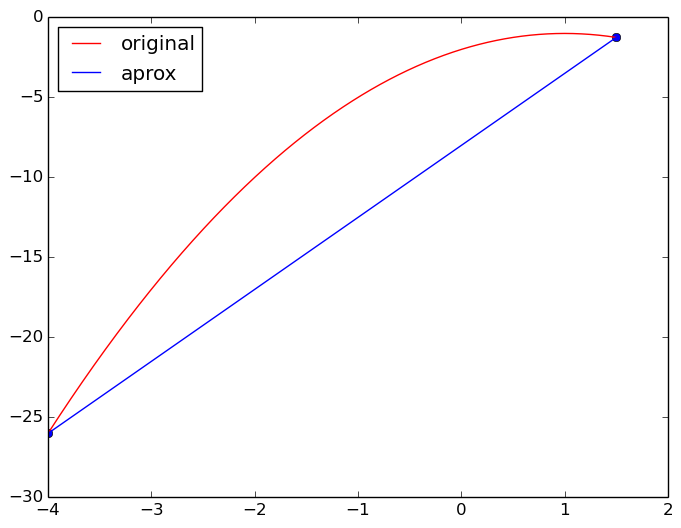
\includegraphics[width=0.3\textwidth,center]{figuras/interpolacao_linear.png}
  \caption{interpolação simples}
\end{figure}
 Para fazermos essa interpolação para $n$ pontos conhecidos aproximamos uma função usando o polinômio base de \emph{Lagrange}.
\begin{equation}
C_i(x) = \prod_{j = 0 \\ j \neq i}^{N} \frac{x - x_j}{x_i - x_j} 
\end{equation}
 A interpolação de \emph{Lagrange} é dada por :
\begin{equation}
 P_n(x) \equiv \sum_{i = 0}^{N} f(x_i)C_i(x) 
\end{equation}
 Obedecendo que $P_n(x_i) = f(x_i)$. Apesar dos pontos interpoladores equidistante serem comumente utilizados, não há restrições, podendo até mesmo estar fora de ordem.
\begin{figure}[h]
  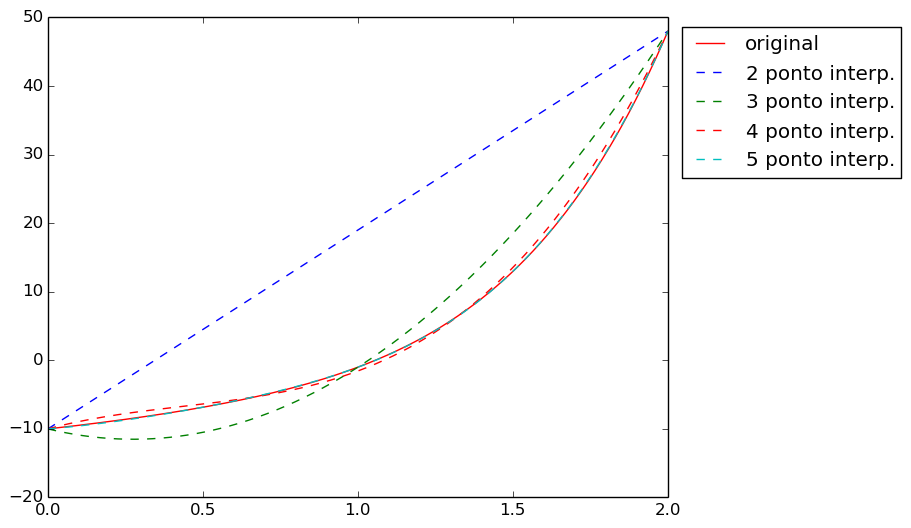
\includegraphics[width=0.4\textwidth, center]{figuras/interpolacao_linear5.png}
  \caption{interpolação com n pontos equidistantes}
\end{figure}


\subsection{Fenômeno de Runge}
 Apesar de parecer que uma boa interpolação tenha uma boa aproximação usando pontos igualmente distantes sobre um interval $[a,b]$, $\lim_{n \rightarrow \infty} |f(x) - P_n(x)| = 0$ para qualquer $f(x)$ diferenciável.
 No início do século XX, \emph{Carl David Tolmé Runge}, provou que para uma função $f(x)$:
 \begin{equation}
 f(x) = \frac{1}{1 + x^2} , x \in [-5,5]
 \end{equation}
 que para pontos equidistantes, a interpolação converge apenas no intervalo $[-3.63,3.63]$, e diverge fora do mesmo. Para polinômios de maior grau, esse intervalo de convergência tende a diminuir e perto dos pontos de fronteira diverge bastante (figura abaixo).

\begin{figure}[!h]
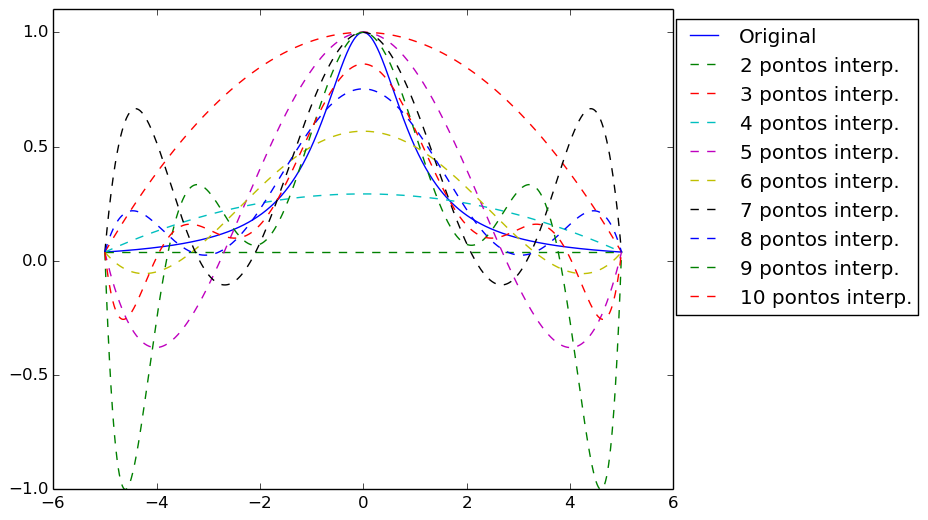
\includegraphics[width=0.4\textwidth, center]{figuras/fenomeno_runge.png}
\caption{fenômeno Runge}
\end{figure}

 Assim, Runge prova que no meio do intervalo temos boas aproximações mas infelizmente perto dos extremos, os valores interpolados oscilam muito, para um polinômio de grau n com pontos equidistante. Esse fenômeno sugere que escolhamos pontos diversos que tenham menor concentração do meio do intervalo, onde temos uma maior precisão, e aumentar a densidade de pontos próximos dos extremos.
 Agora como encontrar uma distribuição de pontos de forma que melhore a interpolação ? A resposta pode ser explicado pelos teoremas a seguir.
 
\subsection{ Teorema I: Erro de interpolação de Cauchy}

 Dado $f(x)$  com pelo menos $N+1$ derivadas no intervalo de interesse e seja $P_N(x)$ seja o interpolador Lagrangiano de grau $N$. Então:
 
 \begin{equation}
 f(x) - P_N(x) = \frac{1}{[N+1]!}f^{(N+1)}(\epsilon)\prod^{N}_{i = 0} (x - x_i)
 \end{equation}
 Para um $\epsilon(x) \in [-1,1]$.
 
  2
test